\documentclass[12pt]{article}

%paquetes del idioma y codificacion
\usepackage[spanish]{babel}
\usepackage[utf8]{inputenc}
\usepackage[T1]{fontenc}
\usepackage{bookman}

%el indice
\usepackage{makeidx}

%paquetes matematicos
\usepackage{amsmath, amsfonts, amssymb}

%dimensiones
\usepackage[left=2.5cm, right=2.5cm, top=3cm]{geometry}

%para escribir codigo
\usepackage{listings}

% para contraer referencias
\usepackage{cite}

%para las imagenes y mas...
\usepackage{graphicx}
\usepackage{subfig}
\graphicspath{ {imagenes/} }
\usepackage{float}


\title{Primer bloque de programas}
\author{Eslí Joana Osorio Rodríguez}


\begin{document}


\maketitle

\newpage

\tableofcontents

\newpage

\section{Introducción}
Este documento contiene la documentación de todos los programas realizados en el primer parcial.
Se dejaron seis programas en total, los resultados obtenidos y los códigos se encuentran a continuación.
Los códigos se encuentran en dos lenguajes C y Python, estos lenguajes los escogí debido a que C es un lenguaje que ya sabia y Python por su facilidad aunque este ultimo lo tuve que aprender.
La forma de programar autómatas es n poco diferente debido a que estos nos dan un resultado analizando estados, no con contadores u otro tipo de herramientas, al principio puede resultar difícil abrir la mente y dejar a un lado la forma en la cual programabas pero después se torna mucho más sencillo y te das cuenta de que muchas veces implementabas cosas que realmente no eran necesarias.


\newpage

\section{Universo}
Un alfabeto básicamente es un conjunto finito de símbolos y es no vacío.
Una cadena es la concatenación de símbolos pertenecientes al alfabeto.
La cadena vacía si existe, no está vacía, pero no tiene símbolos.
 \cite{automatas}

\subsection{Descripción:}
Crear un programa que basado en un alfabeto binario $\sum = \lbrace 0, 1 \rbrace $ ,así el programa debe de ser capaz de mostrarnos todas las combinaciones posibles que se puedan formar con base a el alfabeto el programa está limitado a las potencias $0 \leq n \leq 1000$.

\subsection{Código fuente}
El programa para está problema fue escrito en el lenguaje C\\

Archivo: main.c
\lstset{language=C, breaklines=true, basicstyle=\footnotesize}
\begin{lstlisting}[frame=single]
#include "Random.h"
#include <stdio.h>
#include <stdlib.h>
#include <conio.h>
#include <math.h>


void agregarCaracter(int,int,int,int,char []);
int comenzar(int);
void menu(void);
void Manual(void);
void Automatico(void);
void repetitivo(void);

int main()
{
	menu();
	repetitivo();
}

void menu(void){
	system ("color 8F" );
	int rep;
	int opc=0;
	do{
	printf("\t\tUniverso binario 1\n Seleccione la opcion deseada:\n 1.-Manual \n2..-Automatico\n");
		scanf("%d",&opc);
		//opc=Random(1,2);
		if(opc==1){
		Manual();
		}
		if(opc==2){
		Automatico();
		}
		printf("\n\t\tDesea ingresar otro valor? \n 1.-Si \n 2.- No \n");
		scanf("%d",&rep);
		//rep=Random(0,2)
	}while(rep==1);
	printf("\t\tAdios\n");
}

void repetitivo(void){
	int num=0;
	printf("\nQuieres que se repita? \n 1.Si \n 2. No \n");
	num=Random(1,2);
	if(num==1){
		printf("\n Opcion 1 seleccionada\n");
		menu();
	}else{
		printf("\n Opcion 2 seleccionada, Adios\n");
		return ;
	}
}

void Manual(void){
	int potencia=0;
		printf("\t\tSelecciono el modo Manual\n");
		printf("Incerte la potencia  ");
		scanf("%d",&potencia);
		printf("\nLa potencia insertada es: %d",potencia);
		comenzar(potencia);
		}


void Automatico(void){
	int potencia;
		printf("\t\tSelecciono el modo Automatico\n");
		potencia=Random(0,1000);
		printf("La potencia seleccionada automaticamente= %d",potencia);
		comenzar(potencia);
		
		
}

int comenzar(int potencia){
	FILE *archivo;
	char cadena[potencia];
	int senal;
	senal=potencia;
	int cantidad=pow(2,potencia);
	int contador=1;
	archivo=fopen("archivo.txt","w");
	fprintf(archivo,"A={");
	for(int i=0;i<cantidad;i++){
		int posicion=0;
		
		do{
			if(potencia==0){
				return 0 ;
			}
			else{
				if(potencia==1 && contador%2==1){
					cadena[posicion]='0';
				}
				else{
					if(potencia==1 && contador%2==0){
						cadena[posicion]='1';
					}
					else{
							if(contador<=cantidad/2){
								cadena[posicion]='0';
							}
							else{
								cadena[posicion]='1';
								contador=contador-(cantidad/2);		
								}
					}
				}
			}
			
				
				fprintf(archivo,"%c" ,cadena[posicion]);
			posicion++;
			potencia--;
			
		}while(posicion!=senal);
		
				for(int x=0;x<posicion;x++){
					fprintf(archivo,"%c" ,cadena[x]);
				}
					if(i!=cantidad-1 && i<cantidad){
					fprintf(archivo,",");
					}
					cantidad++;
		}
	fprintf(archivo,"}");
		fclose(archivo);
		return 0;
	}


\end{lstlisting}


\newpage
\subsection{Pruebas}
En cuanto a las pruebas, a continuación se mostraran una serie de imágenes capturadas al momento de ejecutar el programa. Los resultados arrojados por el programa anterior son:

Este programa un no esta del todo bien no gurda bien las cadenas que genera\\

Para la selección en modo automático:

\begin{figure}[H]
\includegraphics[width=\textwidth, height=7cm]{alfabetos_automatico}
\label{fig:auto_alfabeto}
\caption{Selección de un n = 24 de forma automática}
\end{figure}

\vspace{1em}

\begin{figure}[H]
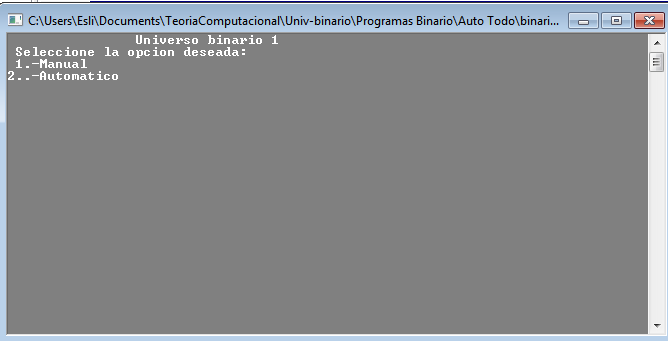
\includegraphics[width=\textwidth, height=6cm]{uni}
\label{fig:Universo}
\caption{Consola}
\end{figure}

\vspace{1em}


%===============================================================================================
%===============================================================================================
%===============================================================================================
%===============================================================================================
%===============================================================================================
%===============================================================================================
%===============================================================================================
%===============================================================================================
\newpage
\section{Números primos}
El conjunto de números primos es infinito, pero números primos solo son aquellos que son divisibles entre ellos mismos y el número uno, para encontrar los números primos no existe ningún algoritmo estables, los números primos no llevan una secuencia ni un patrón por esto hasta la fecha no se existe un algoritmo para saber cuáles son o no primos.

\subsection{Descripción }
Crear un programa que encuentre los números primos dentro del intervalo: $0 \leq n \leq 1000$.Los número primos obtenidos deberán ser guardados en un archivo que contendrá el conjunto decimal y el conjunto binario, después se grafican por el número de ceros y unos de cada número primo en su representación binaria.
\subsection{Código}
El programa está  escrito en C.\\


Archivo: main.py
\lstset{language=C, breaklines=true, basicstyle=\footnotesize}
\begin{lstlisting}[frame = single]
#include "Random.h"
#include <stdio.h>
#include <stdlib.h>
#include <conio.h>
#include <math.h>

int c=0;
int b=0;

void Conversion(int[],int);
int archivarDec(int, int);
void archivarBin(char Numero[], int, int);
void Primos(int);
void Menu();
void Manual();
void Automatico();
int inicializarConjunto(int[]);

int main(int argc, char** argv) {
	system ("color 8F" );
		FILE *fp;
		fp=fopen("archivo.txt","w");
		int rep;
		//Manual();
	
	do{
		rep=0;
		Menu();
		printf ("\t\tDesea ingresar otro valor?\n 1= Si \n 2=No\n");
//		scanf("%d",&rep);
		rep=Random(0,2);
		
	}while(rep==1);
	

	printf ("\t\t Gracias Por su Visita \n\t\t Adios");
}

void Menu(void){
	int opc=0;
	printf("\t\t\t\tNUMEROS PRIMOS\t\t\n MENU :\n 1.- Operacion Manual \n 2.-Operacion automatica\n\n");
//	scanf("%d",&opc);
	opc=Random(0,2);
	if(opc+1==1){
		Manual();
	}
	if(opc+1==2){
		Automatico();
	}
}
void Manual(){
	int limite=0;
		printf("Usted selecciono la forma manual\n");
		printf("introduzca el numero de limite=   ");
		scanf("%d",&limite);
		printf ("\n");
		Primos(limite);
}
void Automatico(){
	printf("Usted selecciono la forma automatica\n");
		int limite=0;
		limite=Random(1,750);
		printf("El numero random del limite es=  %d \n ", limite);
		Primos(limite);
	
	
}

void Coma(){
	FILE *fp;
	fp=fopen("archivo.txt","a");
	fprintf(fp,",");
	
}

void Cerrar(){
	FILE *fp;
		b=0;
		fp=fopen("archivo.txt","a");
		fprintf(fp,"}")	;
		fprintf(fp,"\n")	;
}

int archivarDec(int num, int b){
	int x[130];
	int i;
	x[i]=num;
		FILE *fp;
			if (b==0){
			fp=fopen("archivo.txt","a");
			fprintf(fp,"A={");
			fprintf(fp,"%d" ,x[i]);
			}
			if (b>0){
				fprintf(fp,"%d" ,x[i]);
			}	
	i++;
	return 0;	
}

void archivarBin(char Numero[15], int lim, int ban){
	int bit;
	int a;
		a=lim;
	FILE *fp;
	fp=fopen("archivo.txt","a");
	if (ban ==0)fprintf(fp,"Ab={");
	
	for (a=lim-1; a>=0;a--){
		fprintf(fp,"%d",Numero[a]);
	}
}

int inicializarConjunto(int Conjunto[171]){
	int i;
	for (i=0; i<=127; i++){
		Conjunto [i]=0;
	}
}

void Primos(int limite){
	int num;
	int f=0;
	int conjunto[171];
	int i=0;
	int b=0;
	int c=0;
	int a;
	int bandera;
	inicializarConjunto (conjunto);
				if (limite==0){
				FILE *fp;
				fp=fopen("archivo.txt","a");
				fprintf(fp,"A={e}");
				fprintf(fp,"\n");
				fprintf(fp,"Ab={}");
				fprintf(fp,"\n");
			}
	for (num=1; num<=limite; num++){
		bandera=0;
		for(a=2; a<num; a++){
			if (num%a==0){
				bandera=1;
			}
		}	
		if (bandera==0){
				conjunto [i]=num;
				if (f!=0){
				  Coma();
				}
				archivarDec(num,b);
				c=1;
				b=1;
				f=1;
				i++;
		}
			if (num==limite) {
			Cerrar ();
			Conversion(conjunto,i);
		}
	}
	}
	
void Conversion (int conjunto [171], int lim){
	char numero [10];
	int bit;
	int decimal;
	int i=0;
	int h=0;
	int car;
	int ban=0;
do{
	decimal=conjunto[i];
	h=0;
	do{
		bit= decimal%2;
		numero[h]= (char)bit;
		decimal=decimal/2;
		h++;
	} while (decimal>0);
		i++;
		archivarBin (numero,h,ban);
			if (i!=lim) Coma(); 
		ban=1;
}while (i!=lim);
	Cerrar();
	return ;	
}
\end{lstlisting}

\vspace{1em}


\subsection{Pruebas}
Imagenes del Programa ejecutandose.\\

\begin{figure}[H]
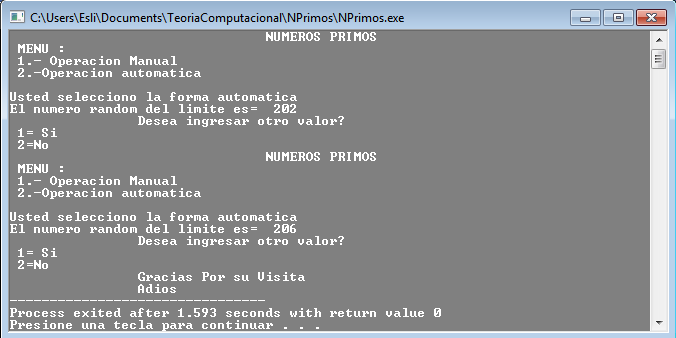
\includegraphics[width=\textwidth, height=13cm]{pautomatico}
\caption{Opción atomática}
\label{fig:par}
\end{figure}
\vspace{1em}

\begin{figure}[H]
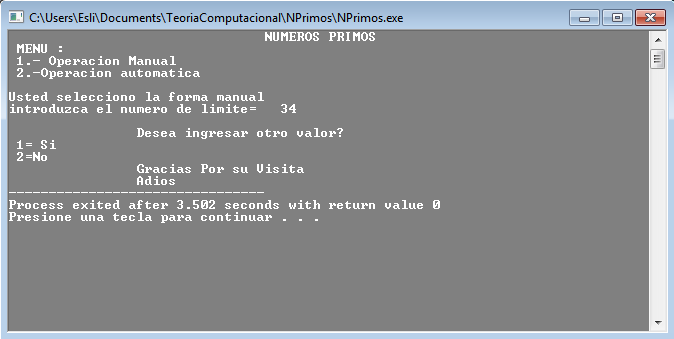
\includegraphics[width=\textwidth, height=10cm]{pmanual}
\caption{Opción manual}
\label{fig:par}
\end{figure}
\begin{figure}[H]
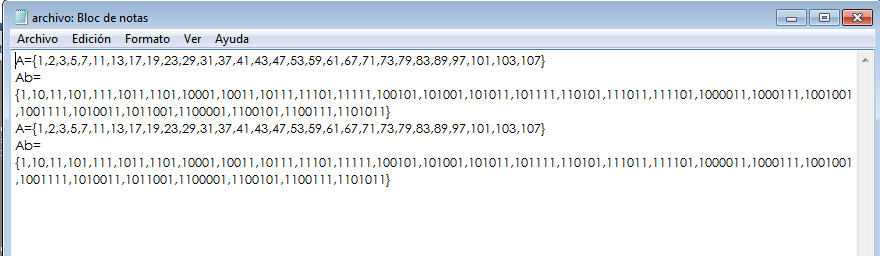
\includegraphics[width=\textwidth, height=10cm]{parchivo}
\caption{Archivo resultante en ambas opciones}
\label{fig:par}
\end{figure}
\begin{figure}[H]
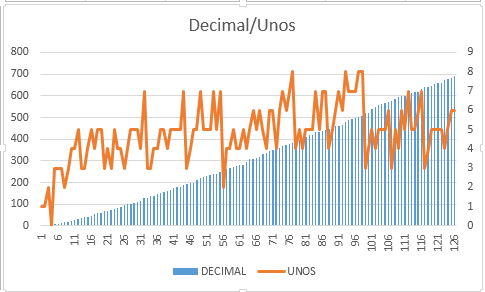
\includegraphics[width=\textwidth, height=10cm]{decimal-unos}
\caption{Gráfica}
\label{fig:par}
\end{figure}
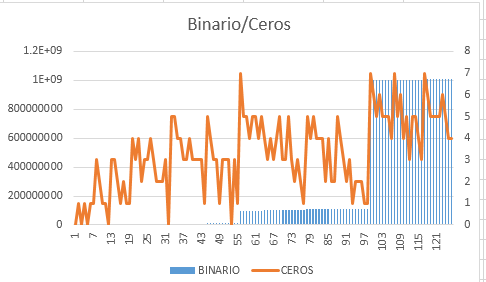
\includegraphics[width=\textwidth, height=10cm]{decimal-ceros}
\caption{Gráfica}
\label{fig:par}
\end{figure}


%===============================================================================================
%===============================================================================================
%===============================================================================================
%===============================================================================================
%===============================================================================================
%===============================================================================================
%===============================================================================================

\newpage
\section{Autómata terinacion -ere}
Los autómatas evalúan a través de estados, un autómata determinístico es aquel que según la entrada asigna un valor, esto quiere decir que todas sus opciones son fijas, este es un autómata sencillo y que ayuda a la comprensión de que son los autómatas y comenzar a implementarlos de una forma sencilla.

\subsection{Descripción }
Crear un autómata que reconoce las cadenas con terminación\textit{ere}. Después vamos almacenar las cadenas validadas, su ubicación y también la ruta que tomo al evaluar las cadenas, debe de ser capaz de analizar todas las posibles opciones que se presenten.

\subsection{Código}
Código fuente del autómata:

\begin{figure}[H]
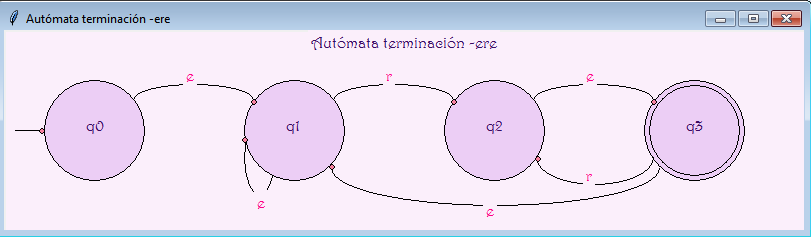
\includegraphics[width=\textwidth, height=10cm]{eregrafico}
\caption{El modelodel autómata es:}
\label{fig:automata-ere}
\end{figure}

El lenguaje utilizado para este programa fue Python\\

Archivo: ere.py
\lstset{language=Python, breaklines=true, basicstyle=\footnotesize}
\begin{lstlisting}[frame=single]
import random 
from tkinter import *
def grafico ():
	ventana=Tk()
	g=Canvas(ventana,bg="#FBEFFB",width=800, height=200)
	g.pack()
	ventana.title("Autómata terminación -ere ")
	ventana.geometry("800x200")
	color="#ECCEF5"
	color1="#380B61"
	etiqueta = Label(ventana, bg="#FBEFFB",text="Autómata terminación -ere",fg=color1, font="Harrington")
	g.create_oval(40,50,140,150, fill=color)
	etiqueta1=Label(ventana, bg=color,text="q0",fg=color1, font="Harrington").place(x=79,y=83)
	g.create_oval(240,50,340,150, fill=color)
	etiqueta2=Label(ventana, bg=color,text="q1",fg=color1, font="Harrington").place(x=279,y=83)
	g.create_oval(440,50,540,150, fill=color)
	etiqueta3=Label(ventana, bg=color,text="q2",fg=color1, font="Harrington").place(x=479,y=83)
	g.create_oval(640,50,740,150, fill=color)
	g.create_oval(645,55,735,145, fill=color)
	etiqueta4=Label(ventana, bg=color,text="q3",fg=color1, font="Harrington").place(x=679,y=83)
	color3="#FF0080"
	color4="#F7819F"
	g.create_arc(10,100,40,100, start=0, extent =180, style='arc')
	g.create_oval(35,97.5,40,102.5, fill=color4)
	g.create_arc(129,85,249,54, start=360, extent =180, style='arc')
	g.create_arc(329,85,449,54, start=360, extent =180, style='arc')
	g.create_arc(529,85,649,54, start=360, extent =180, style='arc')
	g.create_arc(532,100,649,154, start=360, extent =-180, style='arc')
	g.create_arc(327,100,655,175, start=360, extent =-180, style='arc')
	g.create_arc(240,90,270,164, start=332, extent =-180, style='arc')
	g.create_oval(246.5,68.5,251.5,73.5, fill=color4)
	g.create_oval(446.5,68.5,451.5,73.5, fill=color4)
	g.create_oval(646.5,68.5,651.5,73.5, fill=color4)
	g.create_oval(237.5,106.5,242.5,111.5, fill=color4)
	g.create_oval(324.5,133.5,329.5,138.5, fill=color4)
	g.create_oval(530.5,125.5,535.5,130.5, fill=color4)
	etiqueta4=Label(ventana, bg="#FBEFFB",text="e",fg=color3, font="Harrington").place(x=579,y=33)
	etiqueta4=Label(ventana, bg="#FBEFFB",text="r",fg=color3, font="Harrington").place(x=379,y=33)
	etiqueta4=Label(ventana, bg="#FBEFFB",text="e",fg=color3, font="Harrington").place(x=179,y=33)
	etiqueta4=Label(ventana, bg="#FBEFFB",text="r",fg=color3, font="Harrington").place(x=579,y=133)
	etiqueta4=Label(ventana, bg="#FBEFFB",text="e",fg=color3, font="Harrington").place(x=479,y=168)
	etiqueta4=Label(ventana, bg="#FBEFFB",text="e",fg=color3, font="Harrington").place(x=250,y=160)
	g.place(x=0,y=0)
	etiqueta.pack()
	g.mainloop() 
def manual():
		cadena=""
		ubi=open ("Camino.txt","w")
		ubi.close()
		Coordenadas=open ("Coordenadas.txt","w")
		Coordenadas.close()
		print ("\t Usted eligio el modo manual\n Ingrese la cadena porfavor")
		cadena=input ()
		archivo=open ("Entrada.txt","w")
		archivo.write(cadena)
		archivo.close()
		fp=open ("Validado.txt","w")
		fp.close()
		revision(1)
def automatico():
		cadena =""
		ubi=open ("Camino.txt","w")
		ubi.close()
		Coordenadas=open ("Coordenadas.txt","w")
		Coordenadas.close()
		print ("\t Usted eligio el modo automatico")
		archivo=open ("Automatico.txt","r")
		archivo.read()
		archivo.close()
		fp=open ("Validado.txt","w")
		fp.close()
		revision(2)
def revision(j):
	if j==1:
		archivo= open("Entrada.txt","r")
	elif j==2:
		archivo= open("Automatico.txt","r")
	y=0
	for linea in archivo:
		cadena=linea
		estados(cadena,y)
		y=y+1
	archivo.close()
def estados(cadena,y):
	ubi=open ("Camino.txt","a")
	Coordenadas=open ("Coordenadas.txt","a")
	caracter=0
	palabra=cadena.split()
	x=0
	ban1=0
	for i in palabra:
		ban1=0
		tamaño=len(i)
		estado=0
		c=0
		for a in i:		
			if estado==0:
				ubi.write("q0 -"+a+"-->")
				if a=="e" or a=="E":
					estado=1
				else:
					estado=0	
			elif estado==1:
				ubi.write("q1 -"+a+"-->")
				if a=="r" or a=="R":
					estado=2
				elif a=="e" or a=="E":
					estado=1
				else :
					estado=0
			elif estado==2:
				ubi.write("q2 -"+a+"-->")
				if a=="e" or a=="E":
					estado=3
				else:
					estado=0
			elif estado==3:
				if tamaño==c:
					ubi.write("q3 -"+a+"FIN")
					ban1=1
					guardar(i)
					Coordenadas.write("Ubicacion:" + str(y+1) + "," + str(x+1) + "," + str(caracter-c) + "\n")
				elif tamaño==c+1:
					estado=5
				elif a=="r" or a=="R":
					ubi.write("q3 -"+a +"-->")
					estado=2
				elif a=='e' or a=='E':
					ubi.write("q3 -"+a +"-->")
					estado=1
				else:
					estado=0
			elif estado==5:
				if a=="," or a=="." or a=="?" or a=="!" or a=="}" or a=="]" or a==")" or a=="'" :
					guardar(i[0:len(i)-1])
					ubi.write("q3 -"+a+"FIN")
					ban1=1
					Coordenadas.write("Ubicacion:" + str(y+1) + "," + str(x+1) + "," + str(caracter-c) + "\n")		
			c=c+1
		if estado==3:				
				if tamaño==c:
					ubi.write("q3 -"+a+"FIN")
					ban1=1
					guardar(i)
					Coordenadas.write("Ubicacion:" + str(y+1) + "," + str(x+1) + "," + str(caracter-c) + "\n")
				elif tamaño==c+1:
					estado=5
				else:
					estado=0				
		elif estado==5:
				if a=="," or a=="." or a=="?" or a=="!" or a=="}" or a=="]" or a==")" or a=="'" :
					guardar(i[0:len(i)-1])
					ubi.write("q3 -"+a+"FIN")
					ban1=1
					Coordenadas.write("Ubicacion:" + str(y+1) + "," + str(x+1) + "," + str(caracter-c) + "\n")	
		if ban1==0:
			ubi.write("No Valida\n")
		else:
			ubi.write("\n")
		x=x+1
		caracter=caracter+c
def guardar(i):
	palabra=i
	valida=open ("Validado.txt","a")
	valida.write(palabra)
	valida.write(" ")
	valida.close()
def menu():
	entra=1
	while entra==1:
		print("\t\tSeleccione la opcion deseada\n 1.-Manual\n2.-Automatico\n3.-Grafico\n")
		#opc=str(input())
		opc=str(random.randrange(1,4))
		print(opc)
		if opc=='1':
			manual()
		elif opc=='2':
			automatico()
		elif opc=='3':
			print("\t\tFue seleccionado el modo Grafico\n")
			grafico()
		print("desea regresar?\n1.-Si\,2.-No\n")
			#entra=int(input())
		entra=random.randrange(0,2)
	print ("\t\tADIOS\n")

menu()

\end{lstlisting}

\vspace{1em}


\subsection{Pruebas}
Resultados.

\begin{figure}[H]
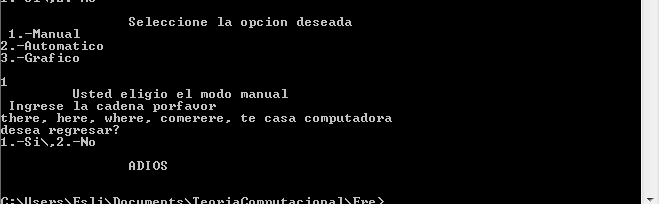
\includegraphics[width=\textwidth, height=8cm]{eremanual}
\caption{consola manual-automático.}
\label{fig:autómata -ere}
\end{figure}
\begin{figure}[H]
\includegraphics[width=\textwidth, height=8cm]{eretext}
\caption{Un texto automático.}
\label{fig:autómata -ere}
\end{figure}

\begin{figure}[H]
\includegraphics[width=\textwidth, height=8cm]{eretextman}
\caption{Un archivo generado de modo manual.}
\label{fig:automata -ere}
\end{figure}

\begin{figure}[H]
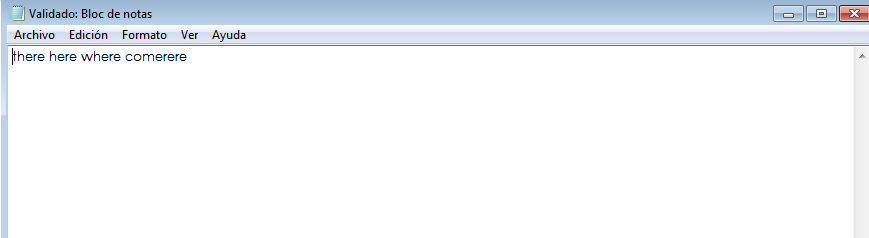
\includegraphics[width=\textwidth, height=8cm]{ereresult}
\caption{Archivo de palabras validadas.}
\label{fig:autómata -ere}
\end{figure}

\begin{figure}[H]
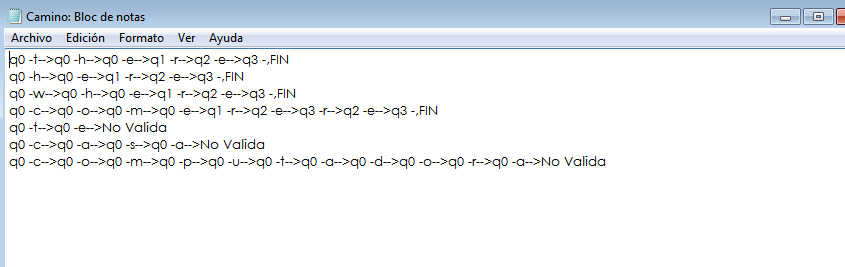
\includegraphics[width=\textwidth, height=8cm]{erecamino}
\caption{Archivo de ruta.}
\label{fig:autómata -ere}
\end{figure}
\begin{figure}[H]
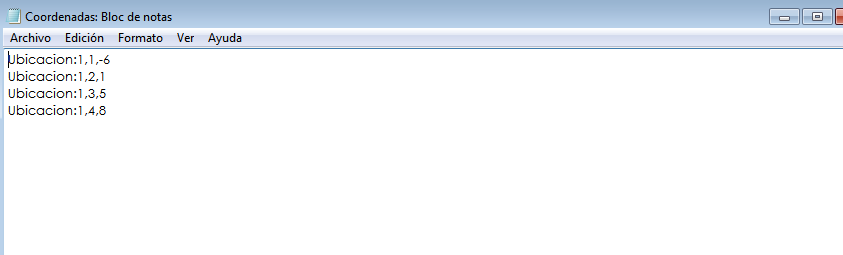
\includegraphics[width=\textwidth, height=8cm]{coordenadas}
\caption{Archivo de coordenadas.}
\label{fig:autómata -ere}
\end{figure}
%------------------------------------------------------------------------
%
%------------------------------------------------------------------------------------
\newpage
\section{Autómata de paridad}
Este autómata sigue siendo determinístico, al ingresar una cadena a de 1's y 0's realmente no sabemos que cantidad de 1's y 0's contiene, no tenemos tampoco una fórmula para contarlos, solamente a mano, para solucionar esto implementaremos un autómata.

\subsection{Descripción }
Crear un autómata que nos verifique si una cadena tiene paridad o sea que su número de 0´s y 1's sea par. Después las cadenas se guardan en un archivo colocándonos ahí cuales son las que tiene paridad y en otro archivo se guardan los estados.


\subsection{Código}
Código fuente:

\begin{figure}[H]
\includegraphics[width=\textwidth, height=10cm]{automata_ere}
\caption{El autómata utilizado para este problema}
\label{fig:automata paridad}
\end{figure}

El lenguaje utilizado para este programa fue Python\\

Archivo: paridad.py
\lstset{language=Python, breaklines=true, basicstyle=\footnotesize}
\begin{lstlisting}[frame=single]
import random 
from tkinter import *
def grafico():
	ventana=Tk()
	g=Canvas(ventana,bg="#FBEFFB",width=500, height=500)
	g.pack()
	ventana.title("Autómata de Paridad ")
	ventana.geometry("400x400")
	color="#ECCEF5"
	color1="#380B61"
	etiqueta = Label(ventana, bg="#FBEFFB",text="Autómata de Paridad",fg=color1, font="Harrington")
	g.create_oval(40,50,140,150, fill=color)
	g.create_oval(45,55,135,145, fill=color)
	etiqueta1=Label(ventana, bg=color,text="q0",fg=color1, font="Harrington").place(x=79,y=83)
	g.create_oval(240,50,340,150, fill=color)
	etiqueta2=Label(ventana, bg=color,text="q1",fg=color1, font="Harrington").place(x=279,y=83)
	g.create_oval(240,250,340,350, fill=color)
	etiqueta3=Label(ventana, bg=color,text="q2",fg=color1, font="Harrington").place(x=79,y=283)
	g.create_oval(40,250,140,350, fill=color)
	etiqueta4=Label(ventana, bg=color,text="q3",fg=color1, font="Harrington").place(x=279,y=283)
	color3="#FF0080"
	color4="#F7819F"
	g.create_arc(10,100,40,100, start=0, extent =180, style='arc')
	g.create_oval(35,97.5,40,102.5, fill=color4)
	g.create_arc(129,85,249,54, start=360, extent =180, style='arc')#arriba
	g.create_arc(129,115,249,146, start=360, extent =-180, style='arc')#abajo
	g.create_arc(240,132,270,265, start=90, extent =180, style='arc')#izquierda
	g.create_arc(310,132,340,265, start=90, extent =-180, style='arc')#derecha
	g.create_arc(129,286,249,255, start=360, extent =180, style='arc')#arriba2
	g.create_arc(129,316,251,347, start=360, extent =-180, style='arc')#abajo2
	g.create_arc(45,132,65,265, start=90, extent =180, style='arc')#izquierda
	g.create_arc(115,132,135,265, start=90, extent =-180, style='arc')#derecha
	g.create_oval(246.5,68.5,251.5,73.5, fill=color4)
	g.create_oval(127,128.5,132,133.5, fill=color4)
	g.create_oval(325.5,262.5,330.5,267.5, fill=color4)
	g.create_oval(251.5,131.5,256.5,136.5, fill=color4)
	g.create_oval(246.5,268.5,251.5,273.5, fill=color4)
	g.create_oval(127,329.5,132,334.5, fill=color4)
	g.create_oval(51.5,261.5,57.5,266.5, fill=color4)
	g.create_oval(123.5,131.5,128.5,136.5, fill=color4)
	etiqueta4=Label(ventana, bg="#FBEFFB",text="1",fg=color3, font="Harrington").place(x=179,y=38)
	etiqueta4=Label(ventana, bg="#FBEFFB",text="1",fg=color3, font="Harrington").place(x=179,y=133)
	etiqueta4=Label(ventana, bg="#FBEFFB",text="0",fg=color3, font="Harrington").place(x=232,y=190)
	etiqueta4=Label(ventana, bg="#FBEFFB",text="0",fg=color3, font="Harrington").place(x=332,y=193)
	etiqueta4=Label(ventana, bg="#FBEFFB",text="0",fg=color3, font="Harrington").place(x=179,y=238)
	etiqueta4=Label(ventana, bg="#FBEFFB",text="0",fg=color3, font="Harrington").place(x=179,y=333)
	etiqueta4=Label(ventana, bg="#FBEFFB",text="1",fg=color3, font="Harrington").place(x=40,y=185)
	etiqueta4=Label(ventana, bg="#FBEFFB",text="1",fg=color3, font="Harrington").place(x=130,y=185)
	g.place(x=0,y=0)
	etiqueta.pack()
	g.mainloop() 
def manual():
		cadena=""
		ubi=open ("Camino.txt","w")
		ubi.close()
		print ("\t Usted eligio el modo manual\n Ingrese la cadena de i's y 0's porfavor")
		cadena=input ()
		archivo=open ("Manual.txt","w")
		archivo.write(cadena)
		archivo.close()
		fp=open ("Validado.txt","w")
		fp.close()
		revision(1)
def automatico():
		cadena =""
		ubi=open ("Camino.txt","w")
		ubi.close()
		print ("\t Usted eligio el modo automatico")
		archivo=open ("Automatico.txt","r")
		archivo.read()
		archivo.close()
		fp=open ("Validado.txt","w")
		fp.close()
		revision(2)
def revision(j):
		if j==1:
			archivo= open("Manual.txt","r")
		elif j==2:
			archivo= open("Automatico.txt","r")
		for linea in archivo:
			cadena=linea
			estados(cadena)
		archivo.close()
def estados(cadena):
	ubi=open ("Camino.txt","a")
	palabra=cadena.split()
	ban2=0
	ban1=0
	for i in palabra:
		ban1=0
		ban2=0
		tamaño=len(i)
		estado=0
		c=0
		for a in (i+","):		
			if estado==0:
				ubi.write("q0 -"+a+"-->")
				if a=="0":
					estado=2
				elif a=="1":
					estado=1
				elif tamaño==c :
					if a=="," or a==".":
						if ban2==0:
							ban1=1
							ubi.write("FIN\n")
							guardar(i[0:len(i)])
						else :
							ban1=1
							ubi.write("FIN\n")
							guardar(i[0:len(i)-1])
				elif tamaño==c+1:
					if a=="," or a==".":
						estado=0
						ban2=1	
			elif estado==1:
				ubi.write("q1 -"+a+"-->")
				if a=="0":
					estado=3
				elif a=="1":
					estado=0
			elif estado==2:
				ubi.write("q2 -"+a+"-->")
				if a=="0":
					estado=0
				elif a=="1":
					estado=3
			elif estado==3:
				if a=="0":
					estado=1
				elif a=="1":	
					estado=2
			if ban1==0 and tamaño==c:
				ubi.write("No Valida\n")
			c=c+1	
def guardar(i):
	palabra=i
	valida=open ("Validado.txt","a")
	valida.write(palabra)
	valida.write("\n")
	valida.close()
def menu():
	entra=1
	while entra==1:
		print("\t\tSeleccione la opcion deseada\n 1.-Manual\n2.-Automatico\n3.-Grafico\n")
		#opc=str(input())
		opc=str(random.randrange(1,4))
		if opc=='1':
			manual()
		elif opc=='2':
			automatico()
		elif opc=='3':
			print("\t\tFue seleccionado el modo Grafico\n")
			grafico()
		print("desea regresar?\n1.-Si\,2.-No\n")
			#entra=int(input())
		entra=random.randrange(0,2)
	print ("\t\tADIOS\n")

menu()
\end{lstlisting}

\vspace{1em}


\subsection{Pruebas}
Resultados.

\begin{figure}[H]
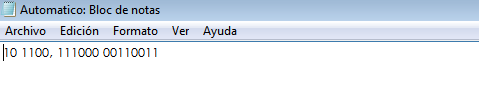
\includegraphics[width=\textwidth, height=8cm]{partxtauto}
\caption{Un texto automático.}
\label{fig:autómata paridad}
\end{figure}

\begin{figure}[H]
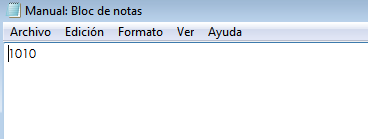
\includegraphics[width=\textwidth, height=8cm]{partxtman}
\caption{Un archivo generado de modo manual.}
\label{fig:autómata paridad}
\end{figure}

\begin{figure}[H]
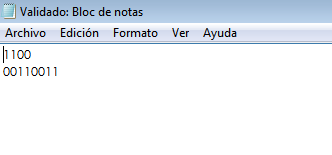
\includegraphics[width=\textwidth, height=8cm]{parresul}
\caption{Archivo de palabras validadas.}
\label{fig:autómata paridad}
\end{figure}

\begin{figure}[H]
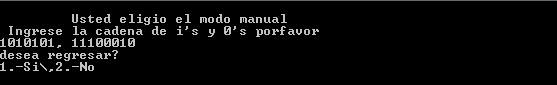
\includegraphics[width=\textwidth, height=8cm]{parmanual}
\caption{Consola manual-automático.}
\label{fig:autómata paridad}
\end{figure}
%--------------------------------------------------------------------------
%
%--------------------------------------------------------------------------------
\newpage

\section{Protocolo}
Este es un protocolo, es un programa totalmente automático, que evalúa tramas de datos.

\subsection{Descripción }
Crear un programa protocolo totalmente automático que en primer lugar pregunte si esta encendido el receptor, si esta encendido crea 50 tramas de 0's y 1's, ya que los recibe el receptor se espera un segundo y pasa por al autómata de paridad y regresa las cadenas validadas y así comienza de nuevo el ciclo hasta que está apagado el receptor.


\subsection{Código}
Código fuente:

\begin{figure}[H]
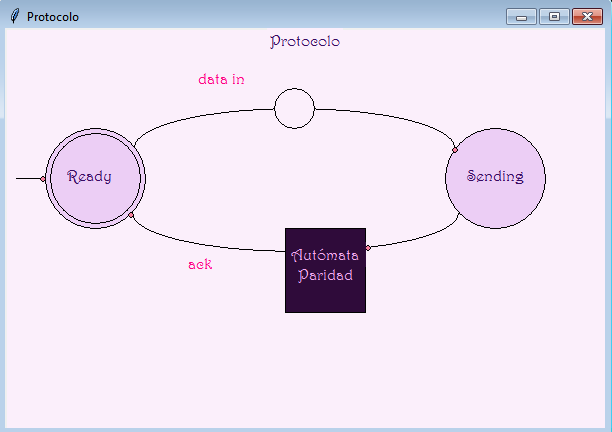
\includegraphics[width=\textwidth, height=10cm]{protocolografico}
\caption{El modelo utilizado para este problema}
\label{fig:protocolo}
\end{figure}

El lenguaje utilizado para este programa fue Python\\

Archivo: protocolo.py
\lstset{language=Python, breaklines=true, basicstyle=\footnotesize}
\begin{lstlisting}[frame=single]
import random 
import time
from tkinter import *
def grafico(encendido):
	ventana=Tk()
	g=Canvas(ventana,bg="#FBEFFB",width=600, height=600)
	g.pack()
	ventana.title("Protocolo")
	ventana.geometry("600x400")
	color="#ECCEF5"
	color1="#380B61"
	etiqueta = Label(ventana, bg="#FBEFFB",text="Protocolo",fg=color1, font="Harrington")
	g.create_oval(40,100,140,200, fill=color)
	g.create_oval(45,105,135,195, fill=color)
	etiqueta1=Label(ventana, bg=color,text="Ready",fg=color1, font="Harrington").place(x=59,y=135)
	g.create_oval(440,100,540,200, fill=color)
	etiqueta2=Label(ventana, bg=color,text="Sending",fg=color1, font="Harrington").place(x=459,y=135)
	color3="#FF0080"
	color4="#F7819F"
	g.create_arc(10,150,40,150, start=0, extent =180, style='arc')
	g.create_oval(35,147.5,40,152.5, fill=color4)
	g.create_arc(129,158,449,80, start=360, extent =180, style='arc')#arriba
	g.create_arc(127,146,453,223, start=360, extent =-180, style='arc')#abajo2
	g.create_oval(446.5,118.5,451.5,123.5, fill=color4)
	g.create_oval(122.5,188.5,127.5,183.5, fill=color4)
	g.create_oval(360,216.5,365,221.5, fill=color4)
	etiqueta4=Label(ventana, bg="#FBEFFB",text="data in",fg=color3, font="Harrington").place(x=190,y=38)
	etiqueta4=Label(ventana, bg="#FBEFFB",text="ack",fg=color3, font="Harrington").place(x=180,y=223)
	if encendido==1:
		g.create_oval(269,60,309,100, fill="#FF0040")
	elif encendido==0:
		g.create_oval(269,60,309,100, fill="#FBEFFB")
	g.create_rectangle(280,200,360,284, fill="#2F0B3A")
	etiqueta4=Label(ventana, bg="#2F0B3A",text="Autómata ",fg="#F5A9F2", font="Harrington").place(x=283,y=214)
	etiqueta4=Label(ventana, bg="#2F0B3A",text="Paridad ",fg="#F5A9F2", font="Harrington").place(x=290,y=234)
	g.place(x=0,y=0)
	etiqueta.pack()
	g.mainloop() 
def creacion():
	archivo=open ("Automatico.txt","w")
	for a in range (50):
		cadena=""
		for i in range(32):
			cadena+=str(random.randrange(0,2))
		archivo.write(str(a)+".-"+cadena+"\n")
def revision():
	archivo= open("Automatico.txt","r")
	for linea in archivo:
		cadena=linea
		estados(cadena)
	archivo.close()
def estados(cadena):
	ubi=open ("Camino.txt","a")
	palabra=cadena.split()
	ban2=0
	ban1=0
	for i in palabra:
		ban1=0
		ban2=0
		tamaño=len(i)
		estado=0
		c=0
		for a in (i+","):		
			if estado==0:
				ubi.write("q0 -"+a+"-->")
				if a=="0":
					estado=2
				elif a=="1":
					estado=1
				elif tamaño==c :
					ban1=1
					ubi.write("FIN\n")
					guardar(i)
			elif estado==1:
				ubi.write("q1 -"+a+"-->")
				if a=="0":
					estado=3
				elif a=="1":
					estado=0
			elif estado==2:
				ubi.write("q2 -"+a+"-->")
				if a=="0":
					estado=0
				elif a=="1":
					estado=3
			elif estado==3:
				if a=="0":
					estado=1
				elif a=="1":	
					estado=2
			if ban1==0 and tamaño==c:
				ubi.write("No Valida\n")
			c=c+1	
def guardar(i):
	palabra=i
	valida=open ("Validado.txt","a")
	valida.write(palabra)
	valida.write("\n")
	valida.close()
def menu():
	archivo=open ("Automatico.txt","w")
	encendido=1
	while encendido==1:
		encendido=random.randrange(0,2)
		camprot=open ("camprot.txt","a")
		if encendido==1:
			grafico(1)
			print ("\t\tEncendido\n")
			camprot.write("Encendido -> ")
			creacion()
			camprot.write("Creacion -> ")
			ubi=open ("Camino.txt","w")
			ubi.close()
			fp=open ("Validado.txt","w")
			fp.close()
			archivo=open ("Automatico.txt","r")
			archivo.read()
			archivo.close()
			print ("\t\tRevision en curso\n")
			camprot.write("Revision -> Fin\n ")
			time.sleep(2)
			revision()
		else:
			grafico(0)
			camprot.write("No encendido \n ")
			print ("\t\tNo esta encendido\n")
		encendido=random.randrange(0,2)
	print ("\t\tYa no esta encendido\n")
	camprot.write("Ya no esta encendido \n ")


menu()
\end{lstlisting}

\vspace{1em}


\subsection{Pruebas}
Imagenes del Programa ejecutandose.\\


\begin{figure}[H]
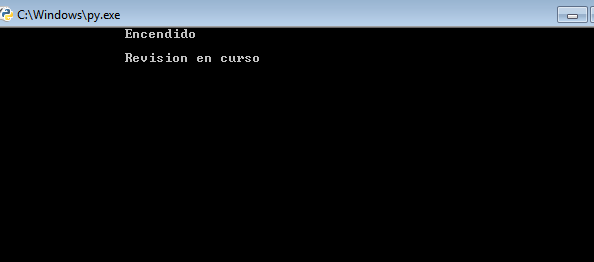
\includegraphics[width=\textwidth, height=13cm]{protocoloconsola}
\caption{consola}
\label{fig:protocolo}
\end{figure}
\vspace{1em}


\begin{figure}[H]
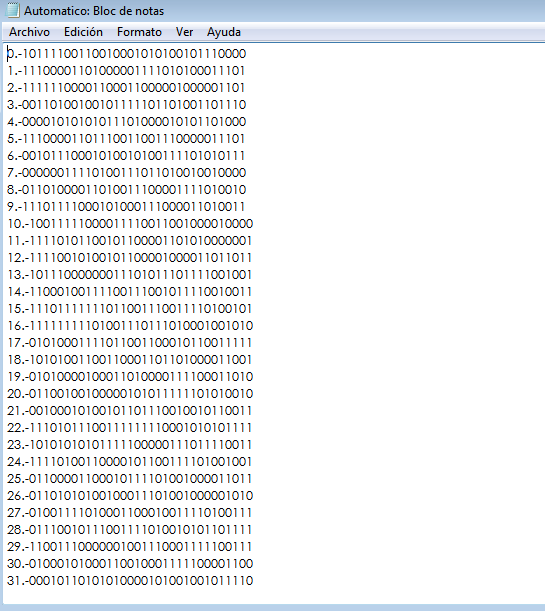
\includegraphics[width=\textwidth, height=10cm]{protocolotxtauto}
\caption{Archivo generado automaticamente}
\label{fig:protocolo}
\end{figure}

\begin{figure}[H]
\includegraphics[width=\textwidth, height=10cm]{protocolotxtcamino}
\caption{Camino con las evaluaciones}
\label{fig:protocolo}
\end{figure}
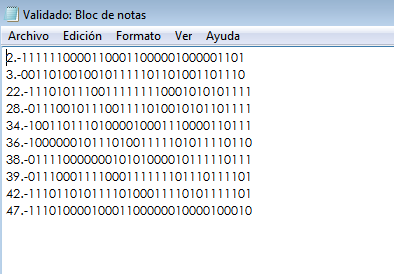
\includegraphics[width=\textwidth, height=10cm]{protocoloresul}
\caption{Archivo final}
\label{fig:protocolo}
\end{figure}


\newpage
\section{Cadenas que terminan en 01}
Este programa no supe como hacerlo, investigue y lo intente pero realmente no supe muy bien como realizarlo


\bibliographystyle{acm}
\bibliography{bibliografia}
"Teoría de Autoómatas y lenguajes de programación", Hopcrof J., Motwain R., Vlimn J., Addison Wsley , 2008

\end{document}